\documentclass[]{exam}
\usepackage{amssymb}
\usepackage[top=1in, bottom=1.5in, left=1in, right=1in]{geometry}
\usepackage{tikz}
\usepackage{pgfplots}
\checkboxchar{$\Box$}
\usepackage{graphicx}
\usepackage{caption}
\usepackage{float}
\usepackage{enumerate}
\usepackage{comment}
\usepackage{multicol}
\usepackage{color}
\CorrectChoiceEmphasis{\color{red}}
\SolutionEmphasis{\color{red}}
\usepackage{advdate}
\usepackage{gensymb}
\usepackage{mathrsfs}
\usetikzlibrary{arrows}


\usepackage{pgfkeys,pgfcalendar}

\newcount\pgfdatecount
\newcommand{\tomorrow}{%
\pgfcalendardatetojulian{\year-\month-\day+1}{\pgfdatecount}
\pgfcalendarjuliantodate{\the\pgfdatecount}{\myyear}{\mymonth}{\myday}
\pgfcalendarmonthname{\mymonth}\space\myday,\space\myyear%
}


\newcommand{\advanceday}[1][1]{
\begingroup
\AdvanceDate[#1]
\today
\endgroup}

\newcommand{\vertex}{\node[vertex]}
\tikzstyle{vertex}=[circle, draw, inner sep=0pt, minimum size=6pt]

\usepackage{lastpage} 
\usepackage{extramarks}
\usepackage{graphicx} 
\usepackage{tikz}
\usepackage{sectsty} 
\usepackage{amsmath,amsfonts,amsthm} 
\usepackage{wrapfig, blindtext}

% Margins
\topmargin=-0.45in
\evensidemargin=0in
\oddsidemargin=0in
\textwidth=6.5in
\textheight=9.0in
\headsep=0.25in 
\numberwithin{equation}{section}
\linespread{1.1} 
\setlength\parindent{0pt} % Removes all indentation from paragraphs
\setlength\answerskip{-.075in}
\setlength\answerlinelength{.5in}
\newcommand{\myitem}{\item[-]}




% HEADER AND FOOTER
\pagestyle{headandfoot}
\runningheadrule
\runningfootrule
\firstpageheader{Kutztown University}{  }{MATH 283 -- Calculus III}
\firstpageheadrule
\runningheader{Desmos Lab 2}{ }{MATH 283}
\firstpagefooter{}{}{} 
\runningfooter{}{}{Page \thepage\ of \numpages}


\newcommand{\assignmentname}{Desmos Lab II} % Assignment title
\newcommand{\coursetitle}{MATH 283 -- Calculus III}
\newcommand{\duedate}{Due: Friday, October 10} % Class/lecture time
\newcommand{\readsections}{Read: Section 12.1-12.2, 13.1-13.3} % Teacher/lecturer
\newcommand{\semester}{Fall 2025}
\title{
\vspace{2in}
\textmd{\textbf{\course:\ \assignmentname}}\\
\normalsize\vspace{0.1in}{\duedate}\\
\vspace{0.1in}\large{\textit{\instructor}}
\vspace{3in}
}
\author{\textbf{Author: \authorname}}
\date{Last Updated: \today}

\pointsinrightmargin
\bracketedpoints


%\printanswers % Unomment this line to Print Solutions 

\begin{document}


%%%%%%%%%%%%%%%%%%%%%%%%%%%%%%%%%%%%%%%%%%%%%%%%%%%%%
% TITLES AND SUCH
%%%%%%%%%%%%%%%%%%%%%%%%%%%%%%%%%%%%%%%%%%%%%%%%%%%%%
\hspace{1in}\\ \vspace{.15in}


\hbox to \textwidth{Name: \hrulefill\hrulefill }

\begin{center}
\normalsize
 \fbox{\fbox{\parbox{5.5in}{

        {\bf Instructions:}  All solutions should be prepared carefully and neatly.  Any questions that ask you to explain or justify should have answers written in complete sentences.  All solution sets shall be completed on this packet and handed in at the beginning of class on the due date below.  Careless presentation (e.g.~bad handwriting, pen scribbles, doodles, wasted space, etc) will result in a deduction of points at my discretion.  If the question asks to submit a graph or plot, be sure to print the plot and include it in your final lab report.  Use a PENCIL and if you make a mistake, use an eraser.  Each student should prepare their own solutions that demonstrate their own comprehension of the material.  Submitted work that does not demonstrate clearly the process by which one arrived at the answer will not receive credit of any kind.  Academic dishonesty will not be tolerated. }}}
\end{center}

\vspace{.5cm}

\ifprintanswers
	\begin{center}
		\Huge\textsc{\assignmentname}\\
		\Large{\textsc{\coursetitle}}\\[4pt]
		\Large\textsc{\color{red}Solution Key
		}
	\end{center}
\else
	\begin{center}
		\Huge\textsc{
		\assignmentname}\\[4pt]
                 \Large{\textsc{\coursetitle}\\[10pt]}
                 \Large{\textsc{\duedate}\\[8pt]}
                 \Large{\textsc{\readsections}\\[8pt]
                 }
	\end{center}
\fi

\Large
\begin{center}
\textsc{\textcolor{red}{Solutions}}
\end{center}


%%%%%%%%%%%%%%%%%%%%%%%%%%%%%%%%%%%%%%%%%%%%%%%%%%%%%
%%%%%%%%%%%%%%%%%%%%%%%%%%%%%%%%%%%%%%%%%%%%%%%%%%%%%


\clearpage
%%%%%%%%%%%%%%%%%%%%%%%%%%%%%%%%%%%%%%%%%%%%%%%%%%%%%
% Blank Page
%%%%%%%%%%%%%%%%%%%%%%%%%%%%%%%%%%%%%%%%%%%%%%%%%%%%%
\normalsize
\
\vspace{.5cm}

\huge
\begin{center}
\begin{tabular}{|c|c|c|}
\hline
Problem  & Available  &   Your  \\
Number & Points &    Points  \\	\hline\hline

 $1$  & 10  & \textcolor{red}{10}  \\	\hline
 $2$  & 10  & \textcolor{red}{10} \\	\hline
 $3$  & 10 & \textcolor{red}{10}  \\	\hline

Total & 30  &  \textcolor{red}{30} \\ \hline
\end{tabular}
\end{center}

\pagebreak

\normalsize
\begin{questions}



%%%%%%%%%%%%%%%%%%%%%%%%%%%%%%%%%%%%%%%%%%%%%%%%%%%%%%%%%%%%
% Question 1 
%%%%%%%%%%%%%%%%%%%%%%%%%%%%%%%%%%%%%%%%%%%%%%%%%%%%%%%%%%%%
\question \underline{Vector-Valued Functions:} In this part, we'll explore a vector-valued function whose graph is traversed by a ``worm.'' We will also compute and interpret the velocity and acceleration vectors, which act as the antenna of the worm.  Then, we'll compute some appropriate metrics of this curve. 
	
\begin{parts}
	\part Open a new graph in Desmos and save it as ``Vector-Valued Functions."
	\part In your Desmos project, create a new folder labeled ``Curve."  In this folder, define three functions on three separate lines: $f(t) = \cos(t)$, $g(t) = \sin(t)$, and $h(t) = t$.  Then, on the fourth line, define the vector valued function $\boldsymbol{r}(t) = \langle f(t), g(t), h(t) \rangle$, for $t\in [0, 10]$.  Plot the curve in grey with width $0.5$.  Describe the curve below. 
	
	\textcolor{red}{The vector-valued function traces out the shape of a helix or spring that is oriented upward with the $z$-axis in the center.  The $z$-axis is essentially the axis of rotation of the helix and the spacing as $t$ increases is constant since $h(t) = t$ is a linear function of $t$.}
	
	
	\part Create a new folder labeled ``Parameters.'' In this folder, define the value $a$ and $b$.  Add them as sliders and allow $a$ to range from $0$ to $10$ and $b$ to range from $1$ to $5$, each with step size $0.1$.  Redefine $f(t) = b\cos(at)$ and $g(t) = b\sin(at)$.  Describe what each parameter does to the curve as it increases.  

	\textcolor{red}{Keeping the window constant, increasing the value of $a$ creates more rotation of the spring because it is increasing the frequency.  This gives the visualization that the spring is compressing as $a$ increases. The parameter $b$ is the amplitude of the periodic functions in $x$ and $y$, which generates a larger circular rotation around the $z$-axis.  In other words, the radius of the helix increases creating a larger spring as $b$ increases. }
	
	\part In the space below, find the \textit{unit velocity vector}, call it $\boldsymbol{T}(t)$, and the \textit{unit acceleration vector}, call it $\boldsymbol{A}(t)$, in terms of $f(t)$, $g(t)$, and $h(t)$.  Create a new folder in Desmos called ``The Worm.'' In this folder, define $T$ as a slider that ranges from $0$ to $10$, with step size $0.001$.  Define a point on the curve at $T$, make it red, with size 6.  In the space below, define a velocity line segment and an acceleration line segment, incorporating the unit vectors $\boldsymbol{T}(t)$ and $\boldsymbol{A}(t)$, that extends out from this point.  Define and graph these segments in this folder, velocity vector in blue and acceleration vector in orange.  Does it make sense why the vectors are pointing the direction they are pointing? Explain. 
	
	\textcolor{red}{We have} 
		\begin{align*}
			\color{red}{\boldsymbol{r}'(t)} & \color{red}{= \langle -ab\sin(at), ab\cos(at), 1\rangle} \\
			\color{red}{\boldsymbol{r}''(t)} & \color{red}{= \langle -a^2b\cos(at), -a^2b\sin(at), 0\rangle} \end{align*}
		\textcolor{red}{and} 
		\begin{align*}
			\color{red}{|\boldsymbol{r}'(t)|} &\color{red}{ = \sqrt{a^2b^2\sin^2(at) + a^2b^2\cos^2(at) + 1} = \sqrt{a^2b^2 + 1}} \\
			\color{red}{|\boldsymbol{r}''(t)|} &\color{red}{ = \sqrt{a^4b^2\cos^2(at) + a^4b^2\sin^2(at) } = \sqrt{a^4b^2}= a^2b}	\end{align*}
			
		\textcolor{red}{Therefore, the unit tangent and acceleration vectors are given by the following vectors: }
		\begin{align*}
			\color{red}{\displaystyle \boldsymbol{T}(t) }&\color{red}{ = \frac{\boldsymbol{r}'(t)}{|\boldsymbol{r}'(t)|} = \left\langle -\frac{ab\sin(at)}{\sqrt{a^2b^2+1}}, \frac{ab\cos(at)}{\sqrt{a^2b^2 + 1}}, \frac{1}{\sqrt{a^2b^2+1}} \right\rangle}\\
			\color{red}{\displaystyle \boldsymbol{A}(t) }&\color{red}{ = \frac{\boldsymbol{r}''(t)}{|\boldsymbol{r}''(t)|} = \left\langle -\cos(at), -\sin(at), 0 \right\rangle}\end{align*}			

		\textcolor{red}{Since $f(t), g(t)$, and $h(t)$ are defined in Desmos, we can simply define the unit tangent vector as }
		\begin{align*}
			\color{red}{\boldsymbol{T}(t) }&\color{red}{ = \frac{1}{\sqrt{f'(t)^2 + g'(t)^2 + h'(t)^2}}\langle f'(t), g'(t), h'(t) \rangle} \\ 
			\color{red}{\boldsymbol{A}(t) }&\color{red}{ = \frac{1}{\sqrt{f''(t)^2 + g''(t)^2 + h''(t)^2}}\langle f''(t), g''(t), h''(t) \rangle }\end{align*} 
			
		\textcolor{red}{Let $T$ be a single value of the parameter $t$.  To create the two line segments, we define the following vector functions in Desmos:}
		\begin{align*}
			\color{red}{\boldsymbol{r_{tan}}(t)} &\color{red}{ = \boldsymbol{r}(T)  + t \boldsymbol{T}(T)} \\  
			\color{red}{\boldsymbol{r_{acc}}(t)} &\color{red}{ = \boldsymbol{r}(T)  + t \boldsymbol{A}(T)} \end{align*}  
		\textcolor{red}{for $t$ ranging from $0$ to $1$. To make the vectors longer, we can make $t$ have a larger upper bound.  The tangent vector is pointing in the direction of motion and the acceleration is pointing almost normal to the motion, inwards toward the axis of rotation.  This makes sense because the tangent vector is in the direction of the velocity, and there exists a force acting on the body towards the center of the helix, so acceleration points inward. }
			
				
	\part To create the body of the worm, create a list in Desmos by typing \texttt{c = [1, 2, ... 20]} on a new line in the worm folder.  Define $h_{step} = 0.01$ on a new line.  Define a set of points as $(f(T-ch_{step}), g(T-ch_{step}), h(T-ch_{step}))$.  Color them green with size 6.  Make your worm crawl along the curve.  
	\part Finally, in a new folder called ``Arc-Length,'' on a new line, have Desmos calculate the arc-length of the curve.  Write the formula below, and type it in almost identically in Desmos.
	
	\textcolor{red}{We are graphing the space curve for $t \in [0, U]$, where $U$ is a real number.  Therefore, the arc-length of the curve is given by 
	\[ \text{Arc-Length} = \int_0^U \left|\boldsymbol{r}'(t)\right|\, dt = \int_0^U \sqrt{f'(t)^2 + g'(t)^2 + h'(t)^2}\, dt\] }
	
	\part Explore some different curves by changing the functions for $f, g,$ and $h$.  When you submit this assignment on D2L, share the url to this graph.  
	
		\textcolor{red}{\texttt{https://www.desmos.com/3d/tue96mbdof}}

		
\end{parts}

\pagebreak 







%%%%%%%%%%%%%%%%%%%%%%%%%%%%%%%%%%%%%%%%%%%%%%%%%%%%%%%%%%%%
% Question 2
%%%%%%%%%%%%%%%%%%%%%%%%%%%%%%%%%%%%%%%%%%%%%%%%%%%%%%%%%%%%
\question \underline{Domains and Limits of Two-Variable Functions:}  In this part, we'll explore a few functions and their domains.  We'll also look into evaluating limits of two-variable functions and see why some limits exist and some limits do not exist. When you submit this assignment on D2L, share the url to this graph. 


\begin{parts}
	\part Open a new graph in Desmos and save it as ``Domains and Limits."
	\part Create a folder called ``Functions -- Domains.''  On separate lines of this folder, define the following functions.  Reserve the top line in Desmos for graphing this function.  Based on the graph of the function, write down the domain and sketch it in the $xy$-plane below: 
		\begin{subparts}
			\subpart $\displaystyle f_1(x,y) = \sqrt{x^2 + y^2 - 4}$
			
			\textcolor{red}{ The domain is everything outside a circle of radius 2, including the boundary: }
			
			\textcolor{red}{$\left\{ (x,y) \, \Big| \, x^2 + y^2 \geq 4 \right\}$}
			
			\begin{center}
			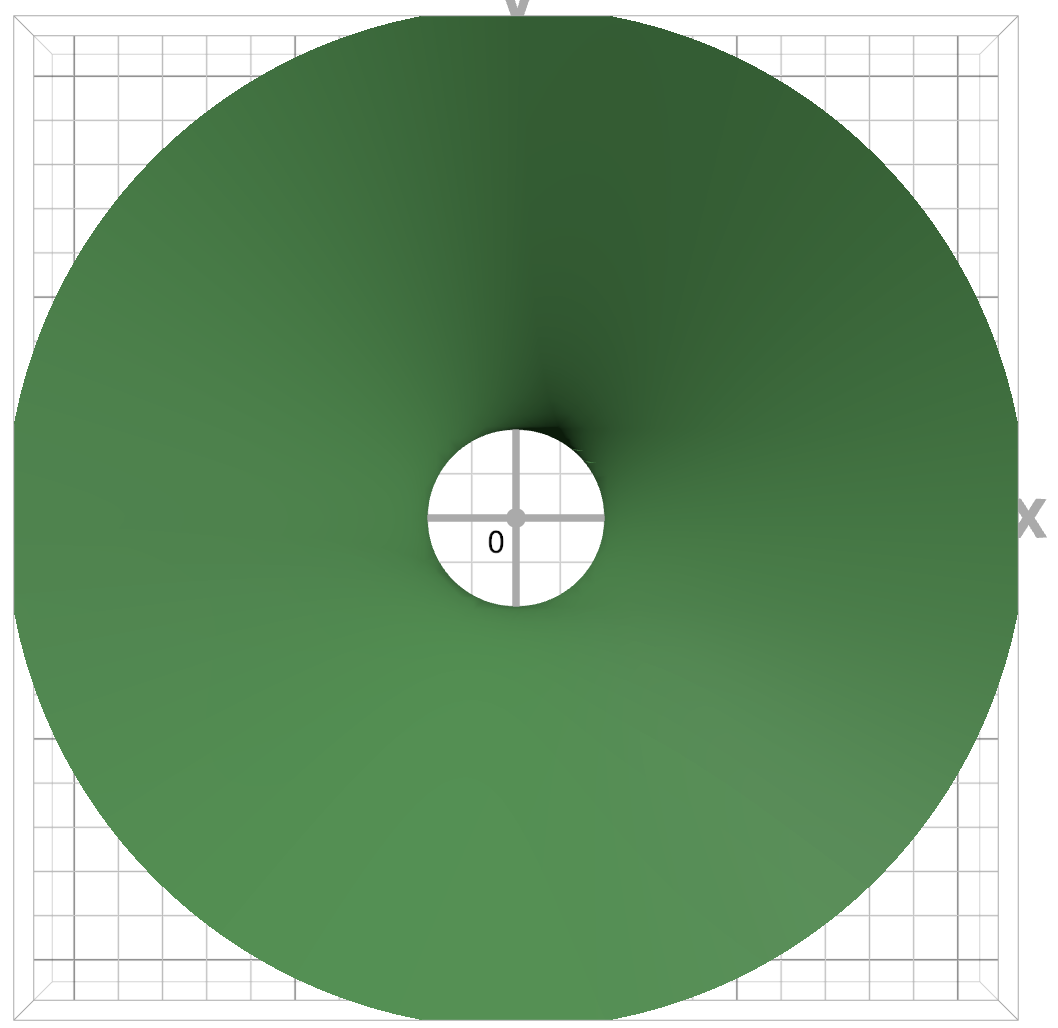
\includegraphics[width = .25\textwidth]{Lab_2_Figure_1.png}
			\end{center}

			\subpart $\displaystyle f_2(x,y) = \sqrt{x-2} + \sqrt{y-1}$

			\textcolor{red}{The domain is $\left\{ (x,y) \, \Big| \, x\geq 2, y\geq 1 \right\}$}

			\begin{center}
			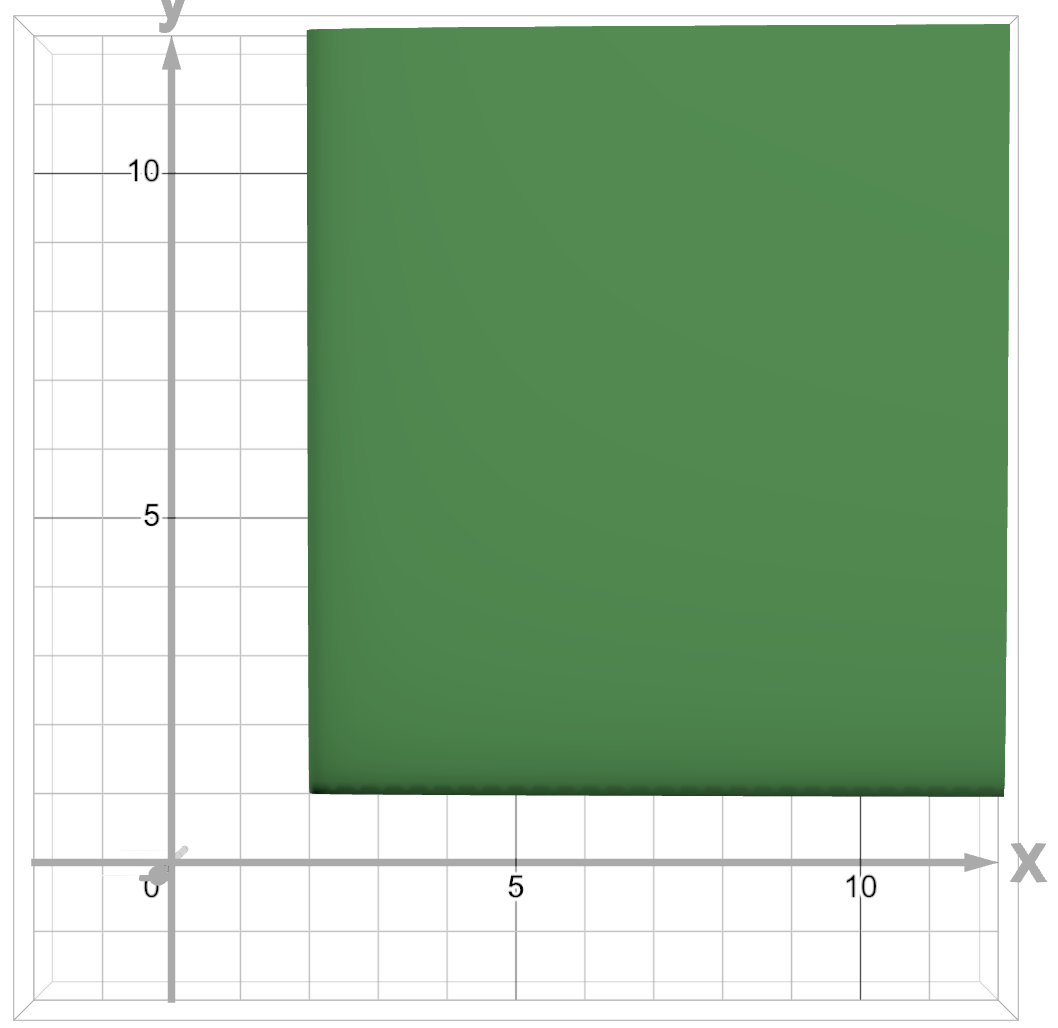
\includegraphics[width = .25\textwidth]{Lab_2_Figure_2.png}
			\end{center}

			\subpart $\displaystyle f_3(x,y) = x\ln(y^2 - x)$

			\textcolor{red}{ The domain is everything to the outside the sideways parabola $x = y^2$: $\left\{ (x,y) \, \Big| \, x\leq y^2 \right\}$}
			
			\begin{center}
			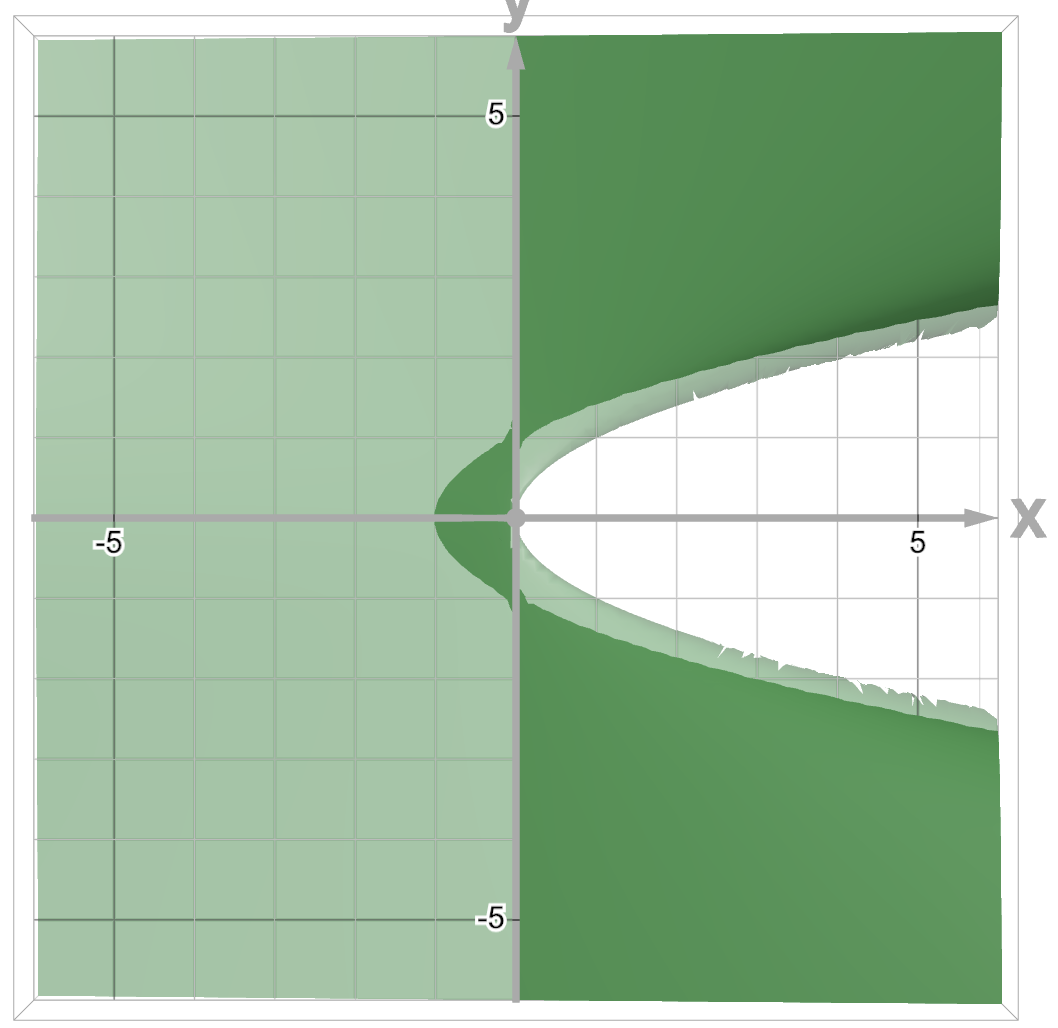
\includegraphics[width = .25\textwidth]{Lab_2_Figure_3.png}
			\end{center}

			\subpart $\displaystyle f_4(x,y) = \frac{\ln(2-x)}{x^2 + y^2 - 1}$

			\textcolor{red}{ The domain is everything to the left of $x = 2$, and it cannot be on the unit circle:} 
			
			\textcolor{red}{$\left\{ (x,y) \, \Big| \, x\leq 2, x^2 + y^2 \neq 1\right\}$}
			
			\begin{center}
			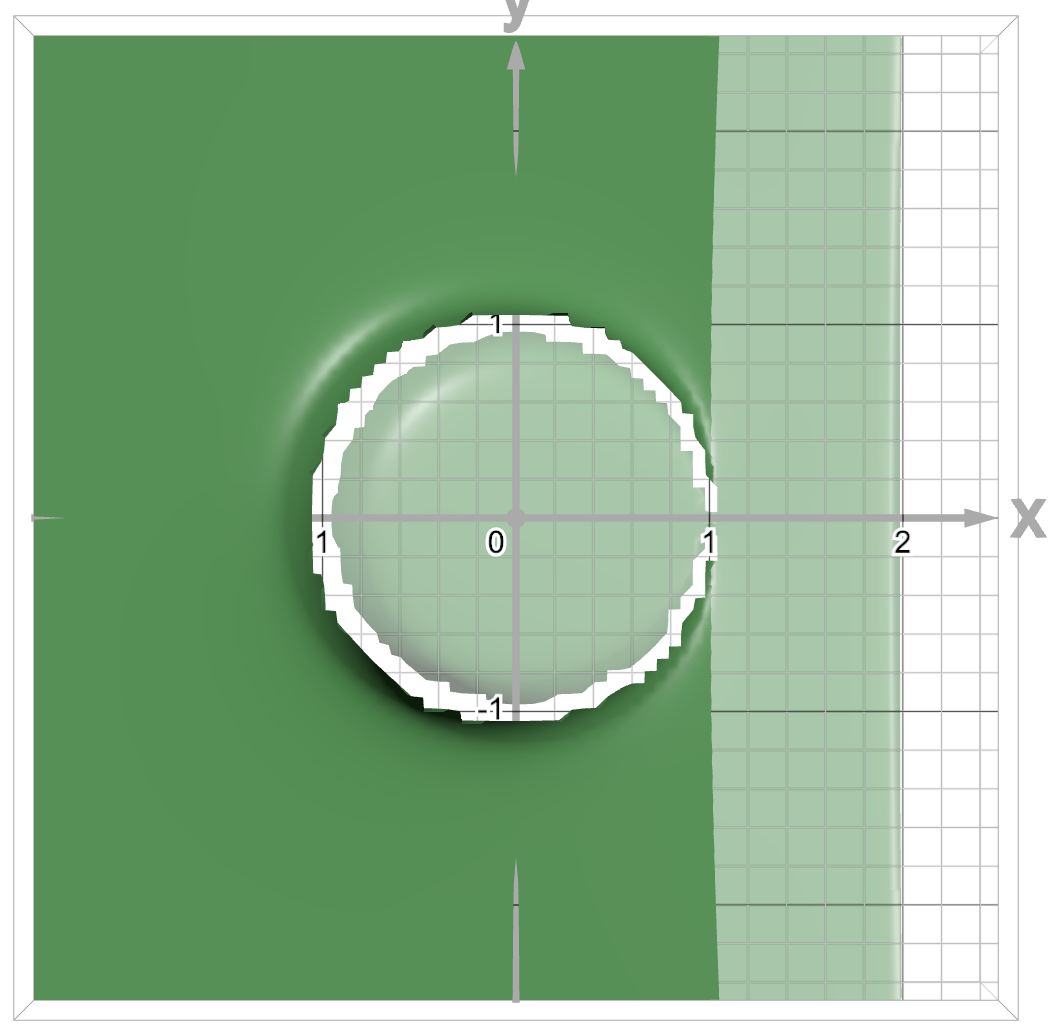
\includegraphics[width = .25\textwidth]{Lab_2_Figure_4.png}
			\end{center}

			\subpart $\displaystyle f_5(x,y) = \frac{\sqrt{x+y+1}}{x-1}$

			\textcolor{red}{ The domain is everything above the line $y = -x-1$ and $x\neq 1$:} 
			
			\textcolor{red}{$\left\{ (x,y) \, \Big| \, y\geq -x-1, x\neq 1 \right\}$}
			
			\begin{center}
			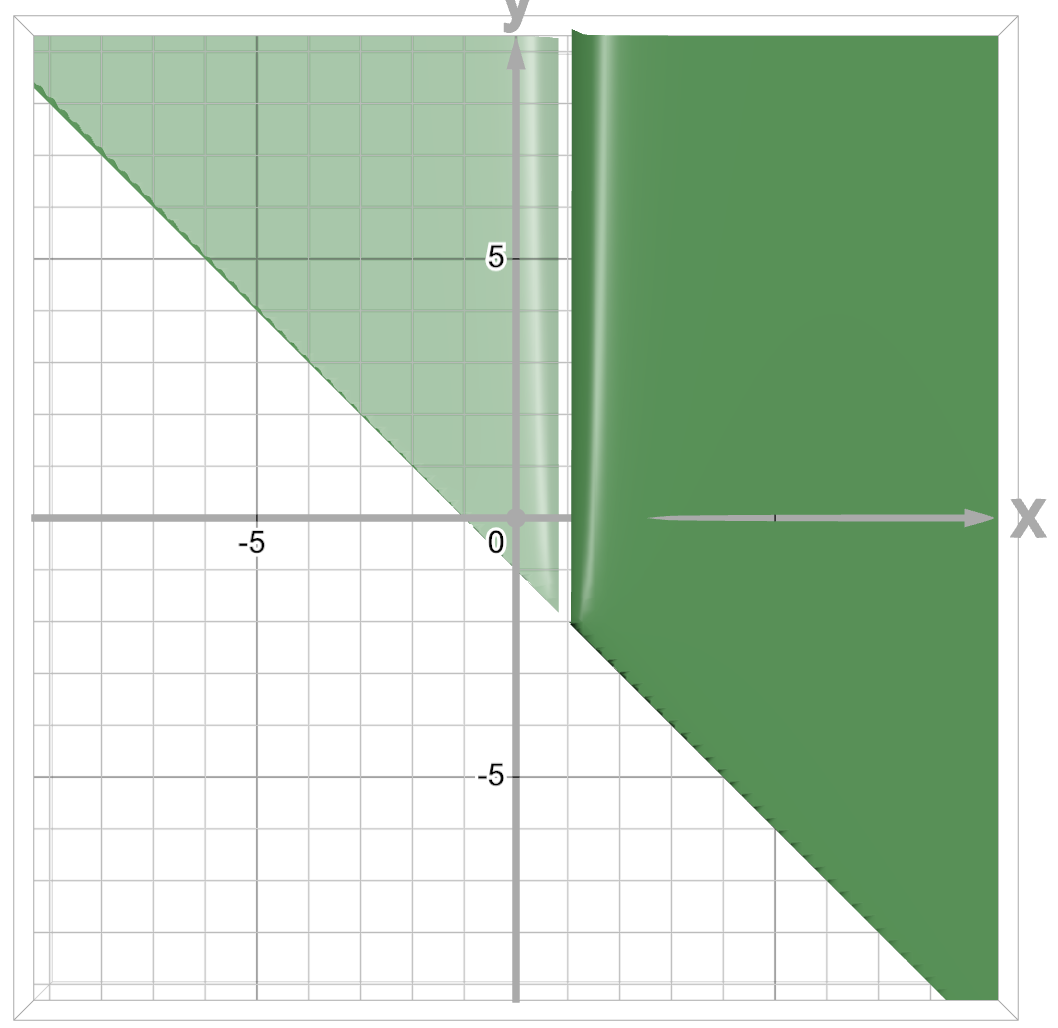
\includegraphics[width = .25\textwidth]{Lab_2_Figure_5.png}
			\end{center}
				
		
		\end{subparts}
		

		\part Create a folder called ``Functions -- Limits.'' On separate lines of this folder, define the following functions, labeling them as $g_1(x,y)$, $g_2(x,y)$, etc.  Based on the graph of the function, determine if the limit exists and write down it's limiting value.  Test different approaches by defining $y$ or $x$ as functions of each other.  If you find two approaches that yield different limiting values, plot both approaches on the surface and write down below the approaches that prove the limit does not exist.  
		\begin{subparts}
			\subpart $\displaystyle \lim_{(x,y) \to (0,0)} \frac{2xy}{x^2 + 3y^2}$ 
			
			\textcolor{red}{Along $y = 0$, the limit is $0$.  Along $y = x$, the limit is $1/2$.  Therefore, the limit doesn't exist. }
			
			\subpart $\displaystyle \lim_{(x,y) \to (0,0)} \frac{y-x}{1 - y + \ln(x)}$

			\textcolor{red}{From the graph of this function, the limit is 0. }
			
			\subpart $\displaystyle \lim_{(x,y) \to (0,0)} \frac{y^2\sin^2(x)}{x^4 + y^4}$

			\textcolor{red}{Along $y = 0$, the limit is $0$.  Along $y = x$, the limit is $1/2$.  Therefore, the limit doesn't exist. }
			
			\subpart $\displaystyle \lim_{(x,y) \to (1,2)} \frac{2x-y}{4x^2 - y^2}$
			
			\textcolor{red}{Along $y = x$, the function is unbounded.  The functions values approach $\infty$ on the positive side and $-\infty$ on the negative side.  Therefore, the limit doesn't exist.   }
			
			\subpart $\displaystyle \lim_{(x,y) \to (0,0)}  \frac{xy}{\sqrt{x^2 + y^2}}$

			\textcolor{red}{Converting to polar coordinates shows that this limit exists and is 0.  }			
				
		\end{subparts}
			
		\part	Define a folder called ``Polar Coords," and define the following vector $(u\cos(v), u\sin(v), g(u\cos(v), u\sin(v)))$, where $g$ is one of the functions below.  Let $u$ be a slider, but let $v$ range from 0 to $2\pi$. Plot this curve on the surface to see if it helps with any limits below.  For at least one of the limits above, convert to polar coordinates and show the limit exists as $r\to 0$ below.
		
		\textcolor{red}{\texttt{https://www.desmos.com/3d/phyxkwru2l}}

		
\end{parts}





\pagebreak






%%%%%%%%%%%%%%%%%%%%%%%%%%%%%%%%%%%%%%%%%%%%%%%%%%%%%%%%%%%%
% Question 3
%%%%%%%%%%%%%%%%%%%%%%%%%%%%%%%%%%%%%%%%%%%%%%%%%%%%%%%%%%%%
\question \underline{Tangent Lines and the Tangent Plane:} In this part, we'll explore how to plot tangent lines using partial derivatives.  Then, we'll construct the tangent plane at a point using the direction vector of each tangent line.  

\begin{parts}
	\part Open a new graph in Desmos and save it as ``Tangent Lines and the Tangent Plane."
	\part Define the function $\displaystyle f(x,y) = 10y^2\sin(x)e^{-x^2 - y^2}$ on the first line in Desmos. On the next two lines, define $a$ and $b$ as constants.  
	\part In the space below, write down the vector form of the tangent line that is parallel to the $xz$-plane in terms of the partial derivative $f_x$ at $(a,b)$.  Define this line and plot it in Desmos, defining each element in a new folder called ``xz-Plane Tangent.'' Also plot the cross-sectional slice in grey for $y = b$.
	
	\textcolor{red}{$\boldsymbol{r_{xz}}(t) = \langle a, b, f(a,b)\rangle + t \langle 1, 0, f_x(a,b)\rangle$}
	
	\part In the space below, write down the vector form of the tangent line that is parallel to the $xz$-plane in terms of the partial derivative $f_y$ at $(a,b)$.  Define this line and plot it in Desmos, defining each element in a new folder called ``yz-Plane Tangent.'' Also plot the cross-sectional slice in grey for $x = a$. 
	
	\textcolor{red}{$\boldsymbol{r_{yz}}(t) = \langle a, b, f(a,b)\rangle + t \langle 0, 1, f_y(a,b)\rangle$}
	
	\part Create a new folder called ``Tangent Plane."  Using the direction vectors from the tangent lines above, what would be the normal vector for the tangent plane at the point $(a,b, f(a,b))$?  Derive it below, then write down the equation for the this plane.  Define this plane in Desmos, and graph it.
	
	\textcolor{red}{Because the tangent plane contains both tangent lines described above, the normal vector to the tangent plane must be orthogonal to the direction vectors of each tangent line.  There, denoting the normal vector as $\boldsymbol{n}$, we have 
	\[ \boldsymbol{n} = \langle 1, 0, f_x(a,b) \rangle \times \langle 0, 1, f_y(a,b) \rangle = \langle -f_x(a,b), -f_y(a,b), 1\rangle \] }
	\textcolor{red}{Since the point $(a,b,f(a,b))$ lies on the curve and the plane, we have }
		\begin{align*}
		 \color{red}{\boldsymbol{n}\cdot\langle x - a, y- b, z - f(a,b)\rangle} & \color{red}{ = 0} \\
		  \color{red}{\langle -f_x(a,b), -f_y(a,b), 1\rangle \cdot \langle x - a, y- b, z - f(a,b)\rangle} & \color{red}{= 0} \\ 
		  \color{red}{-f_x(a,b)(x-a) - f_y(a,b)(y-b) + z - f(a,b)} & \color{red}{ = 0} \end{align*}
		 \textcolor{red}{Solving for $z$ gives 
		 \[ z = f(a,b) + f_x(a,b)(x-a) + f_y(a,b)(y-b). \]}
	
	\part Explore different functions and vary the point $(a,b)$. When you submit this assignment on D2L, share the url to this graph.  
	
	\textcolor{red}{\texttt{https://www.desmos.com/3d/jxxkrxofcb}}


\end{parts} 








\end{questions}


\end{document} 














